\documentclass{../homework}
\usepackage{ dsfont }
\usepackage{ float }
\usepackage{ mathtools }
\usepackage{ commath }
\usepackage{ physics }

\name{Timothy Devon Morris}
\course{Me En 537}
\term{Fall 2018}
\hwnum{6}

\begin{document}
    \begin{parts}[n]
        \part{} Work the following problems from Spong
       \begin{parts}
           \part{} Let $m$ be the mass of a rectangular solid with sides $a$, $b$ and $c$.
           If the origin is at the center of this solid, we have the following interia tensor
           \[
               I_{\text{com}} = 
               \begin{bmatrix}
                   \frac{m}{12} \left(b^2 +  c^2\right) & 0 & 0 \\
                   0 & \frac{m}{12} \left( a^2 + c^2 \right) & 0 \\
                   0 & 0 & \frac{m}{12} \left( a^2 + b^2 \right)
               \end{bmatrix}
           \]
           Using the parallel axis theorem we can transport this inertia tensor to the edge of the rectangular solid. Thus we have
           \[
               I_{0} = I_{\text{com}} - m[r]_{\times}^2
           \]
           Where $r = [a/2, b/2, c/2]^T$. Thus we have
           \[
               \begin{aligned}
                   I_0 &= 
                   I_{\text{com}} -
                   m \begin{bmatrix}
                   0 & -c/2 & b/2 \\
                   c/2 & 0 & -a/2 \\
                   -b/2 & a/2 & 0
                   \end{bmatrix}
                   \begin{bmatrix}
                   0 & -c/2 & b/2 \\
                   c/2 & 0 & -a/2 \\
                   -b/2 & a/2 & 0
                   \end{bmatrix}
                   \\
                       &=
                   I_{\text{com}}
                   - m
                   \begin{bmatrix}
                       -b^2/4 - c^2/4 & ab/4 & ac/4 \\
                       ab/4 & -a^2/4 - c^2/4 & bc/4 \\
                       ac/4 & bc/4 & -a^2/4 - b^2/4
                   \end{bmatrix}
                   \\
                       &=
                       \begin{bmatrix}
                           \frac{m}{3}(b^2 + c^2) & -\frac{m}{4}ab & -\frac{m}{4}ac \\
                           -\frac{m}{4}ab & \frac{m}{3}(a^2 + c^2) & -\frac{m}{4}bc \\
                           -\frac{m}{4}ac & -\frac{m}{4}bc & \frac{m}{3}(b^2 + c^2)
                       \end{bmatrix}
               \end{aligned}
           \]
           \part{}
           Note that the mass matrix can be written as
           \[
               M(q) = \sum_{i=1}^{N} m_iJ_{v\text{com},i}^TJ_{v\text{com},i} + J_{\omega\text{com},i}\ ^0R_{i,\text{com}} I_i \left( \ ^0R_{i,\text{com}} \right)^T J_{\omega\text{com},i}
           \]
           It suffices to show that $x^TM(q)x > 0$ for any $x \neq 0$. We first note that $I_i$ is a postive definite matrix so we can create the weighted norm $x^TI_ix = \norm{x}_{I_i} > 0$. Thus we have that
           \[
               \begin{aligned}
                   x^TM(q)x &= \sum_{i=1}^{N} m_ix^TJ_{v\text{com},i}^TJ_{v\text{com},i}x + x^TJ_{\omega\text{com},i}\ ^0R_{i,\text{com}} I_i \left( \ ^0R_{i,\text{com}} \right)^T J_{\omega\text{com},i}x \\
                            &= \sum_{i=1}^{N} m_i\norm{J_{v\text{com}}x}^2 + \norm{ \left(\ ^0R_{i,\text{com}}\right)^TJ_{\omega\text{com},i}x }_{I_i}
               \end{aligned}
           \]
           At point we have the sum of many positive components, which will be positive. Thus we have $x^TM(q)x > 0$ and $M(q)$ is positive definite.
           \part{}
           Consider a 3-link cartesian manipulator with prismatic joints in z, then y, then x and assume the links are rectangular.
           \begin{parts}[r]
               \part{} The inertia tensor for each link at its center of mass is
               \[
                   I_i = \begin{bmatrix}
                       \frac{17}{(12)16} & 0 & 0 \\
                       0 & \frac{17}{(12)16} & 0 \\
                       0 & 0 & \frac{1}{(6)16}
                   \end{bmatrix}
               \]
               \part{}
               First we need to calculate jacobians at the center of mass. We note that there is no rotational motion in this system so we have that $J_{\omega\text{com},i} = 0$. So we will proceed to calculate $J_{v\text{com},i}$
               \[
                   J_{v\text{com},1} = 
                   \begin{bmatrix}
                       0 & 0 & 0 \\
                       0 & 0 & 0 \\
                       1 & 0 & 0 
                   \end{bmatrix}
               \]
               \[
                   J_{v\text{com},2} = 
                   \begin{bmatrix}
                       0 & 0 & 0 \\
                       0 & 1 & 0 \\
                       1 & 0 & 0
                   \end{bmatrix}
               \]
               \[
                   J_{v\text{com},3} = 
                   \begin{bmatrix}
                       0 & 0 & 1 \\
                       0 & 1 & 0 \\
                       1 & 0 & 0
                   \end{bmatrix}
               \]
               Now we have that
               \[
                   \begin{aligned}
                       M(q) &= (1)J_{v\text{com},1}^TJ_{v\text{com},1} + (1)J_{v\text{com},2}^TJ_{v\text{com},2} +(1)J_{v\text{com},1}^TJ_{v\text{com},3} \\
                            &= 
                            \begin{bmatrix}
                                1 & 0 & 0 \\
                                0 & 0 & 0 \\
                                0 & 0 & 0
                            \end{bmatrix}
                            +
                            \begin{bmatrix}
                                1 & 0 & 0 \\
                                0 & 1 & 0 \\
                                0 & 0 & 0
                            \end{bmatrix}
                            +
                            \begin{bmatrix}
                                1 & 0 & 0 \\
                                0 & 1 & 0 \\
                                0 & 0 & 1
                            \end{bmatrix}
                            \\
                            &= 
                            \begin{bmatrix}
                                3 & 0 & 0 \\
                                0 & 2 & 0 \\
                                0 & 0 & 1
                            \end{bmatrix}
                   \end{aligned}
               \]
               \part{}
               We first note that the christoffel symbols are given by
               \[
                   c_{ijk} = \frac{1}{2} \left( \pdv{d_{kj}}{q_i} + \pdv{d_{ki}}{q_i} - \pdv{d_{ij}}{q_k} \right)
               \]
               where $d_{ij} = [M(q)]_{ij}$. Since our mass matrix is constant (i.e. it has no dependence on $q$) we have that $c_{ijk} = 0 \ \forall i,j,k$. In terms of the dynamic equations this makes sense becuase this robot consists only of linear motions and therefore should have no coriolis terms.
               \part{} Now we are only missing our gravity. We first start by writing our potential energy
               \[
                   P = P_1 + P_2 + P_3 = 3(9.81)q_1
               \]
               Thus we have that
               \[
                   G(q) = \pdv{P}{q} = \begin{bmatrix}
                       29.43 \\
                       0 \\
                       0
                   \end{bmatrix}
               \]
               So we have the following equation
               \[
                   \begin{bmatrix}
                       3 & 0 & 0 \\
                       0 & 2 & 0 \\
                       0 & 0 & 1
                   \end{bmatrix}\ddot{q} + \begin{bmatrix}
                       29.43 \\
                       0 \\
                       0
                   \end{bmatrix}
                   =
                   \begin{bmatrix}
                       f_1 \\
                       f_2 \\
                       f_3
                   \end{bmatrix}
               \]
           \end{parts}
           \part{} See \texttt{prob1d.m}
       \end{parts}

       \part{} See \texttt{prob2.m}
        \begin{figure}[H]
            \centering
            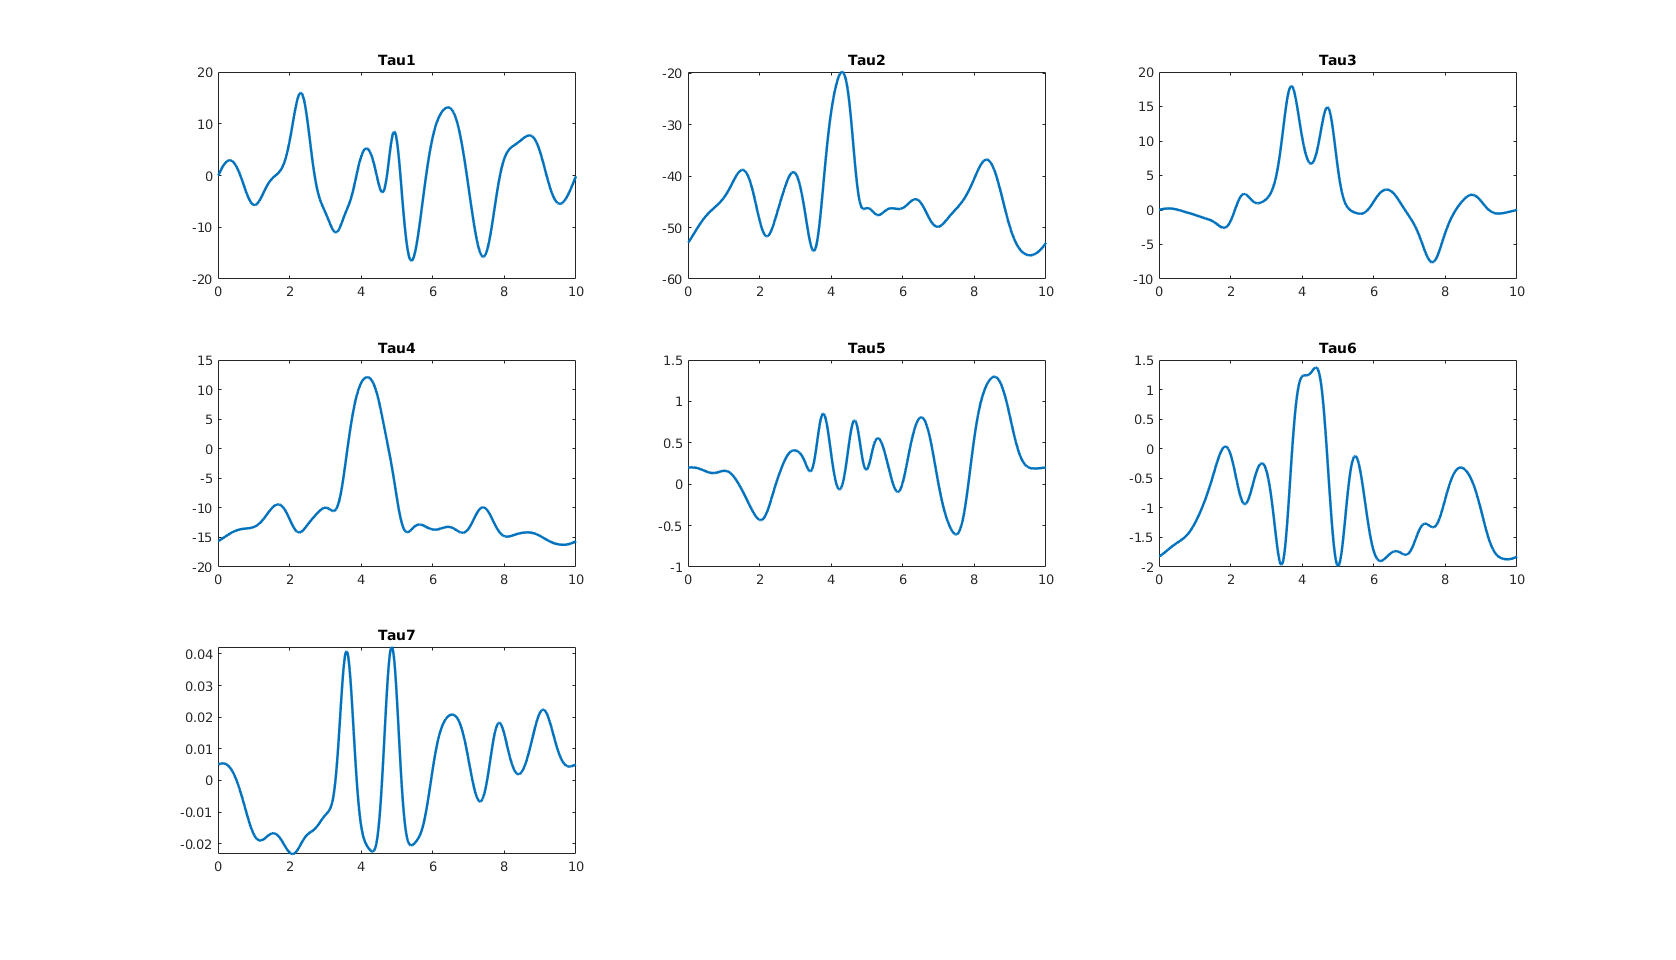
\includegraphics[scale=.3]{prob2.png}
            \label{torq}
            \caption{Torques for Baxter Left Arm}
       \end{figure}

   \end{parts}
\end{document}
